\section{Introduction}
Most of the world's blind people have lost the eye or the optic nerve, so devices that stimulate the retina cannot help them. A cortical visual prosthesis skips that pathway. A camera image is turned into electrical microstimulation of primary visual cortex (V1), and each stimulated site produces a \emph{phosphene}: a small spot of light at the visual-field location that site represents. The idea is old \citep{dobelle2000artificial,schmidt1996feasibility}. Several recent results make it practical:
\begin{itemize}
\item a 96-channel Utah array in a blind volunteer evoked stable phosphenes and allowed letter discrimination \citep{fernandez2021visual};
\item 1024 channels in macaque V1/V4 produced shapes and letters \citep{chen2020shape};
\item dynamic current steering produced form vision in blind humans \citep{beauchamp2020dynamic};
\item thread-based implants now carry thousands of channels \citep{musk2019integrated}, and a thread-based visual prosthesis (Neuralink's ``Blindsight'') received FDA Breakthrough Device designation in 2024.
\end{itemize}

A device with $\sim$1000 sites has an engineering problem in software: the \emph{stimulus encoder}, which maps each camera frame to a vector of per-electrode currents. A good encoder must:
\begin{enumerate}
\item respect how V1 works: cortical magnification, current-dependent phosphene size, detection thresholds and saturation;
\item stay within strict safety limits on current and on the number of electrodes active at once;
\item cope with the fact that each implanted person is different, with dead electrodes, varying thresholds and uncertain phosphene locations;
\item run in real time on wearable hardware.
\end{enumerate}
There is no public human V1 stimulation dataset, so the field works with biologically grounded simulators \citep{vandergrinten2024towards,beyeler2017pulse2percept} and trains encoders end to end through them \citep{deruyter2022end,granley2022hybrid}.

\paragraph{Contributions.}
\begin{enumerate}
\item A fast, differentiable re-implementation of the biologically plausible cortical phosphene model of \citet{vandergrinten2024towards}, with three additions:
  \begin{itemize}
  \item an exact closed form for a single stimulation train that includes within-train habituation;
  \item a separable exact renderer and a two-anchor basis renderer that make CPU training practical;
  \item a patient sampler, and Utah-like and thread-like electrode layouts.
  \end{itemize}
  We check it against published magnification, brightness and threshold data (\S\ref{sec:sim}).
\item A position-aware learned encoder. A small U-Net is read out at each phosphene location, so its parameter count does not depend on electrode count, and a per-electrode gain/bias \emph{patient adapter} sits on top. It is trained through the simulator with a reconstruction, percept-similarity and charge objective, under hard safety limits shared with all baselines.
\item An evaluation on five held-out simulated patients covering MNIST digits, EMNIST letters and CIFAR-10. It reports image similarity, a learned-observer recognition proxy, charge use and robustness to electrode failure, plus ablations over loss terms, safety limits and electrode layout (one Utah array to 1024 sites).
\item Website-ready artefacts: electrode tables with the exact rendering formula and a numeric test case, the baseline algorithm, and the learned encoder in ONNX (all exported from the same code).
\end{enumerate}
All numbers come from CPU-scale runs in the accompanying repository. Where scale limits a conclusion we say so, and \S\ref{sec:repro} describes the full-scale configuration.

\section{Background}
\paragraph{Retinotopy.} V1 maps the contralateral hemifield roughly log-polarly \citep{schwartz1977spatial}. We use the wedge-dipole model \citep{polimeni2006multi} with the human parameters of \citet{vandergrinten2024towards}:
\begin{equation}
  w = k\log\frac{b\,(z_\alpha + a)}{a\,(z_\alpha + b)},\qquad z_\alpha = r e^{i\alpha\theta},
  \label{eq:wedge}
\end{equation}
with $k{=}17.3$\,mm, $a{=}0.75^\circ$, $b{=}120^\circ$ and $\alpha{=}0.95$. Here $r$ is eccentricity, $\theta\in(-\pi/2,\pi/2)$ is polar angle, and $w$ is the cortical position in mm. Along the horizontal meridian the linear magnification is $M(r)=k\,(1/(r{+}a)-1/(r{+}b))$\,mm/deg. For small $r$ this is the \citet{horton1991representation} estimate $17.3/(r+0.75)$. So a fixed cortical spacing gives dense phosphenes near fixation and sparse ones in the periphery.

\paragraph{Phosphenes from microstimulation.} Direct activation spreads roughly as $I=Kr^2$ \citep{tehovnik1996electrical}. With $K{=}675$\,\textmu A/mm$^2$ \citep{tehovnik2006direct,tehovnik2007phosphene}, a current $I$ activates a disc of radius $\sqrt{I/K}$. The phosphene's visual size is that cortical extent divided by $M$, which explains why size grows with eccentricity \citep{winawer2016linking,bosking2017saturation}. Bosking et al.\ also showed that size saturates with current. Intracortical phosphenes are mostly reported as small ``pin-points'' \citep{schmidt1996feasibility,fernandez2021visual}. Their detection thresholds vary between electrodes (66.8$\pm$36.5\,\textmu A in \citealp{fernandez2021visual}), and they fade under repeated stimulation \citep{schmidt1996feasibility}. Microstimulation recruits sparse, distributed populations \citep{histed2009direct}, so phosphene models are phenomenological.

\paragraph{Encoders.} The usual encoders downsample image intensity or edges to the electrode grid. Scene simplification by saliency or segmentation helps in simulated retinal prosthesis users \citep{han2021deep}. End-to-end approaches train a CNN encoder through a differentiable simulator with a decoder or task head \citep{deruyter2022end,kucukoglu2022optimization}. Others invert a patient-specific forward model \citep{granley2022hybrid} or tune encoder parameters from a patient's pairwise preferences \citep{granley2023human}. Retinal percepts are elongated along axon bundles \citep{beyeler2019model}. Cortical percepts are compact blobs, so cortical simulators use Gaussian phosphenes \citep{vandergrinten2024towards}.

\section{A differentiable cortical phosphene simulator}\label{sec:sim}
\paragraph{Electrodes and patients.}
\begin{itemize}
\item Each electrode $n$ has a cortical position in one hemisphere. Inverting Eq.~\eqref{eq:wedge} gives its eccentricity $r_n$ and visual-field centre $(x_n,y_n)$; the left hemisphere represents the right field.
\item A \emph{patient} is a draw of three perturbations:
  \begin{itemize}
  \item cortical position jitter (s.d.\ 0.4\,mm);
  \item dead electrodes (10\%);
  \item per-electrode activation thresholds $A^{\mathrm{thr}}_n\sim\mathcal N(\theta_{50},\sigma_\theta^2)$, clipped at 0, with the values fitted by \citet{vandergrinten2024towards} to \citet{fernandez2021visual}.
  \end{itemize}
\item Encoders only know the \emph{nominal} (planned) positions. The calibrated baselines also know each patient's thresholds and dead electrodes, as they would after a clinical mapping session.
\end{itemize}

\paragraph{Activation and brightness.} Following \citet{vandergrinten2024towards}, a biphasic pulse train with amplitude $I$, pulse width $PW{=}170$\,\textmu s and frequency $f{=}300$\,Hz has effective current
\begin{equation}
I_{\mathrm{eff}} = \max\!\big(0,\,(I - I_0 - B)\,PW\,f\big),
\end{equation}
where $I_0{=}23.9$\,\textmu A is the rheobase leak and $B$ is a habituation trace with $\dot B=\kappa I_{\mathrm{eff}}$ and $\kappa{=}13.96$. Tissue activation integrates this current with a leak, $\dot A=-A/\tau+I_{\mathrm{eff}}$, $\tau{=}0.111$\,s. Within one train of length $T$ the trace's own decay ($\tau_B\approx$\,2000\,s) is negligible. Starting from rest, the coupled system then has an exact closed form, which we use for static frames:
\begin{equation}
A(T) = (I-I_0)\,PW f\;\frac{e^{-\kappa PW f\, T}-e^{-T/\tau}}{1/\tau - \kappa PW f}.
\label{eq:closed}
\end{equation}
With $T{=}166$\,ms (the train of \citealp{fernandez2021visual}), Eq.~\eqref{eq:closed} matches Euler integration of the full dynamics to within 1\% (unit-tested). A phosphene appears only if $A>A^{\mathrm{thr}}_n$. Its brightness is then $b_n=\mathrm{sigmoid}(\lambda(A-A_{50}))$. Because Eq.~\eqref{eq:closed} is linear in $I-I_0$, the threshold current $I^{\mathrm{thr}}_n$ has a closed form, which the calibrated baselines use.

\paragraph{Size and rendering.} The activated radius is $\rho=\sqrt{I/K}$. The phosphene diameter is $P=2\rho/M(r_n)$, rendered as a Gaussian with $2\sigma=P$, as in the eLife text; the released dynaphos code uses half this $\sigma$. We add a fixed display blur in quadrature, $\sigma_{\mathrm{tot}}=\sqrt{\sigma^2+\sigma_{\mathrm{floor}}^2}$ with $\sigma_{\mathrm{floor}}=0.15^\circ$, so that sub-pixel phosphenes neither alias nor vanish at our 64-pixel, $12^\circ$ field of view. The percept is
\begin{equation}
\Phi(x,y)=\operatorname{clip}_{[0,1]}\sum_n b_n\,e^{-\frac{(x-x_n)^2+(y-y_n)^2}{2\sigma_{\mathrm{tot},n}^2}}.
\label{eq:render}
\end{equation}
Each isotropic Gaussian factorises into $x$ and $y$ profiles, so the exact render is one batched matrix product $(B{\times}H{\times}N)\cdot(B{\times}N{\times}W)$ with $O(BN(H{+}W))$ memory. For training we use a faster \emph{basis renderer}:
\begin{itemize}
\item precompute each electrode's Gaussian at two anchor currents (mean threshold and $I_{\max}$);
\item blend the two linearly in current, which needs two dense $(B{\times}N)\cdot(N{\times}HW)$ products;
\item the error against the exact renderer is $<0.03$ per pixel (unit-tested), and evaluation always uses the exact renderer.
\end{itemize}
The detection threshold is a hard step in the forward pass. In training, gradients flow through a sigmoid surrogate (a straight-through estimator), so training and evaluation see the same percepts.

\paragraph{Layouts.} We compare four layouts:
\begin{itemize}
\item \textbf{Utah 96}: a single 10$\times$10 Utah array (0.4\,mm pitch, corners inactive) centred near $2^\circ$ eccentricity \citep{maynard1997utah,fernandez2021visual};
\item \textbf{16$\times$Utah 1024}: sixteen 8$\times$8 arrays split over both hemispheres, at the scale of \citet{chen2020shape};
\item \textbf{threads-64, threads-256} and \textbf{threads-1024}: $N$ independent insertion sites spread with uniform cortical density by best-candidate sampling \citep{mitchell1991spectrally} over $0.2$--$6^\circ$ of both hemispheres.
\end{itemize}
The thread layout is our idealisation of a robot-placed, flexible-thread implant. It is not a device specification. Uniform cortical density automatically produces the magnification-weighted visual-field density shown in Fig.~\ref{fig:layouts}.

\paragraph{Validation.} Figure~\ref{fig:sim} and \texttt{results/validation.json} check the simulator against published data:
\begin{itemize}
\item our magnification agrees with \citet{horton1991representation} to within \NumMagErr\% over $0$--$10^\circ$;
\item at 80\,\textmu A the phosphene diameter is \NumSizeOne$^\circ$ at $1^\circ$ and \NumSizeFive$^\circ$ at $5^\circ$ eccentricity, i.e.\ pin-points, consistent with the intracortical reports;
\item brightness against current for a 166\,ms train reproduces the digitised Fig.~6A of \citet{fernandez2021visual} with $R^2=\NumBrightRsq$;
\item fifty trains 4\,s apart reduce peak brightness by \NumHabDrop\%, qualitatively matching the attenuation reported by \citet{schmidt1996feasibility}. Brightness does not recover during the following 200\,s pauses, because the trace decays with a time constant of about 2000\,s; the recovery dynamics are therefore not validated.
\end{itemize}
One mismatch is clear. The threshold distribution implied by the fitted parameters has mean \NumThrMean\,\textmu A (s.d.\ \NumThrSd), lower than the 66.8\,\textmu A mean of \citet{fernandez2021visual}. We keep the published fit and flag the discrepancy (\S\ref{sec:limits}). For coverage, the fraction of the central field lying within $0.5^\circ$ of some phosphene is \NumCovUtahNine\% for one Utah array, \NumCovUtahThou\% for 16 Utah arrays, \NumCovThrTwo\% for 256 thread sites and \NumCovThrThou\% for 1024 thread sites.

\begin{figure*}[t]
\centering
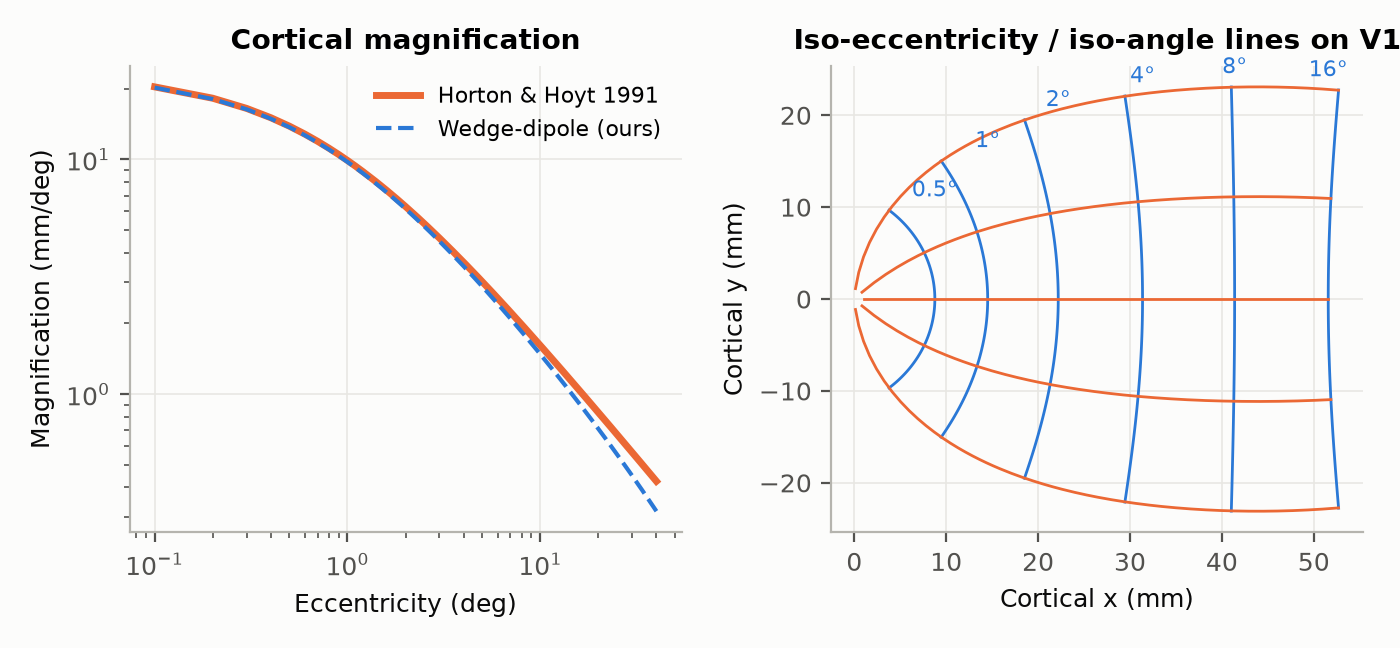
\includegraphics[width=0.49\textwidth]{fig_sim_magnification.png}\hfill
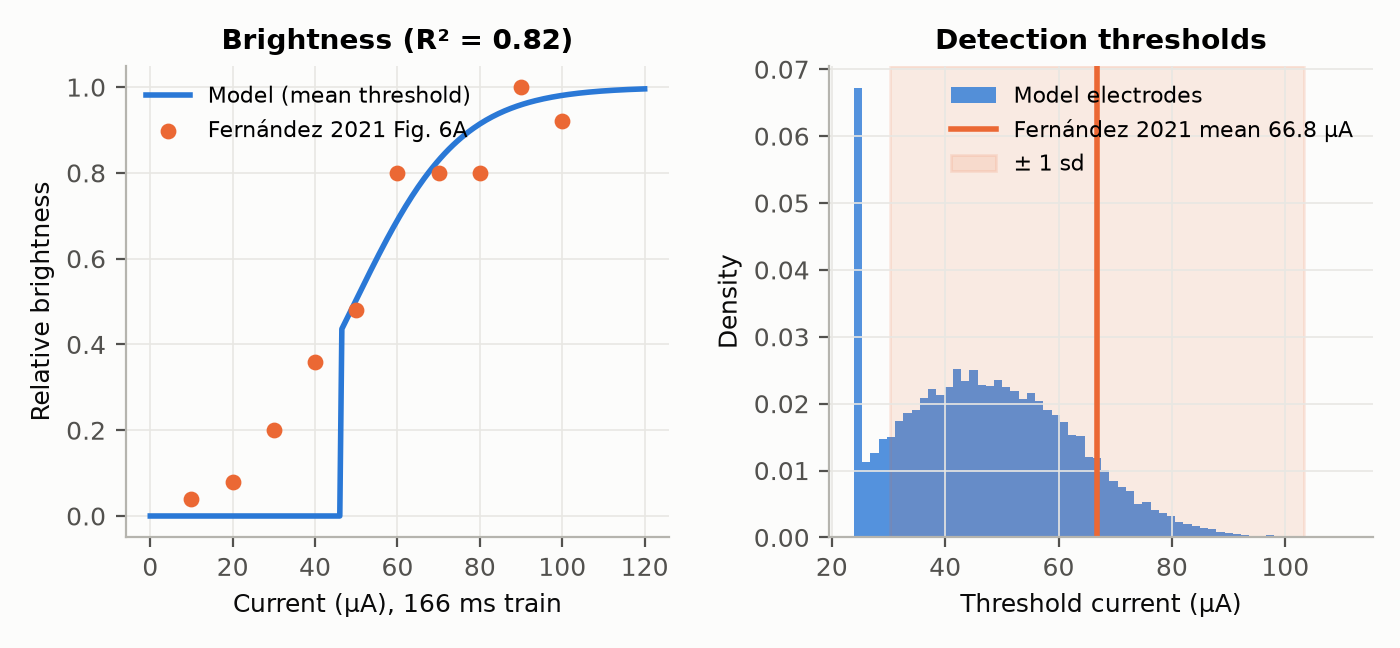
\includegraphics[width=0.49\textwidth]{fig_sim_brightness_threshold.png}\\[2pt]
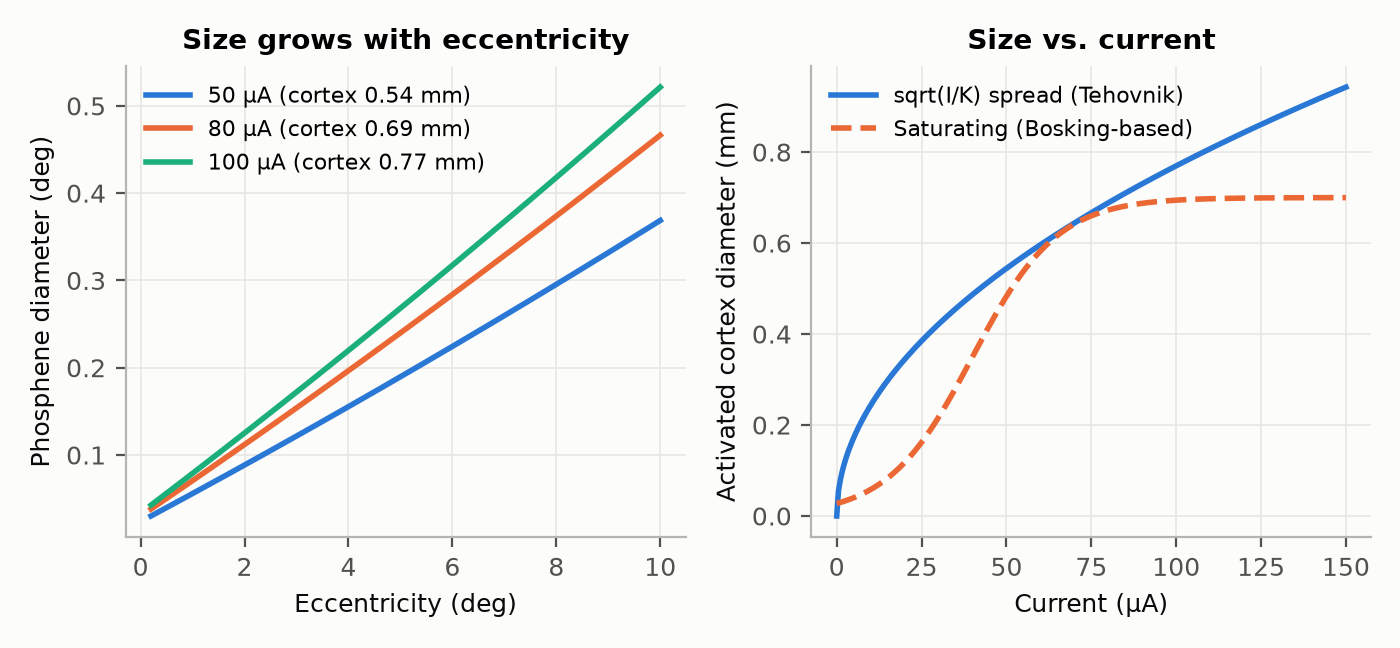
\includegraphics[width=0.49\textwidth]{fig_sim_size.png}\hfill
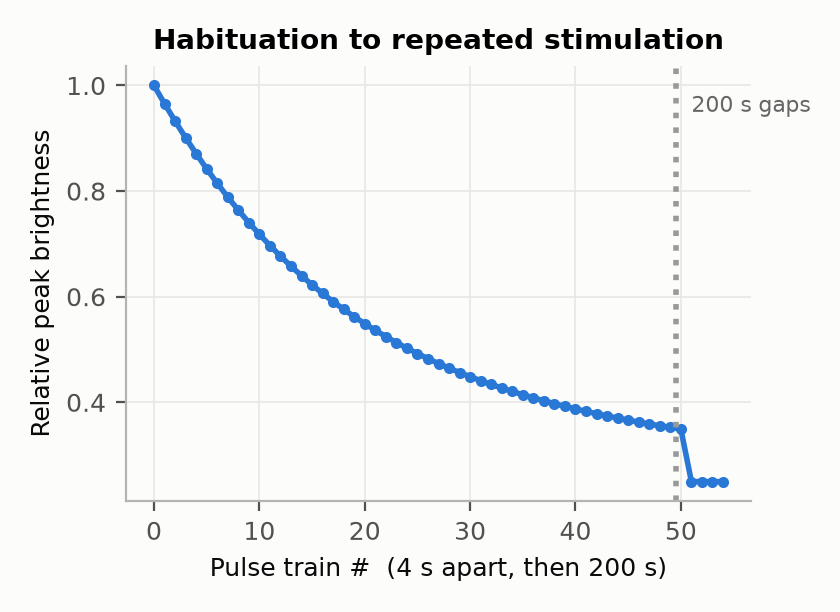
\includegraphics[width=0.30\textwidth]{fig_sim_habituation.png}\hspace*{0.1\textwidth}
\caption{Simulator validation.
\textbf{Top left:} wedge-dipole magnification against \citet{horton1991representation}, and the cortical map.
\textbf{Top right:} brightness against current compared with \citet{fernandez2021visual} Fig.~6A; threshold distribution compared with their reported mean $\pm$ s.d.
\textbf{Bottom:} phosphene size against eccentricity and current, including the saturating Bosking-based alternative; habituation under repeated trains.}
\label{fig:sim}
\end{figure*}

\begin{figure*}[t]
\centering
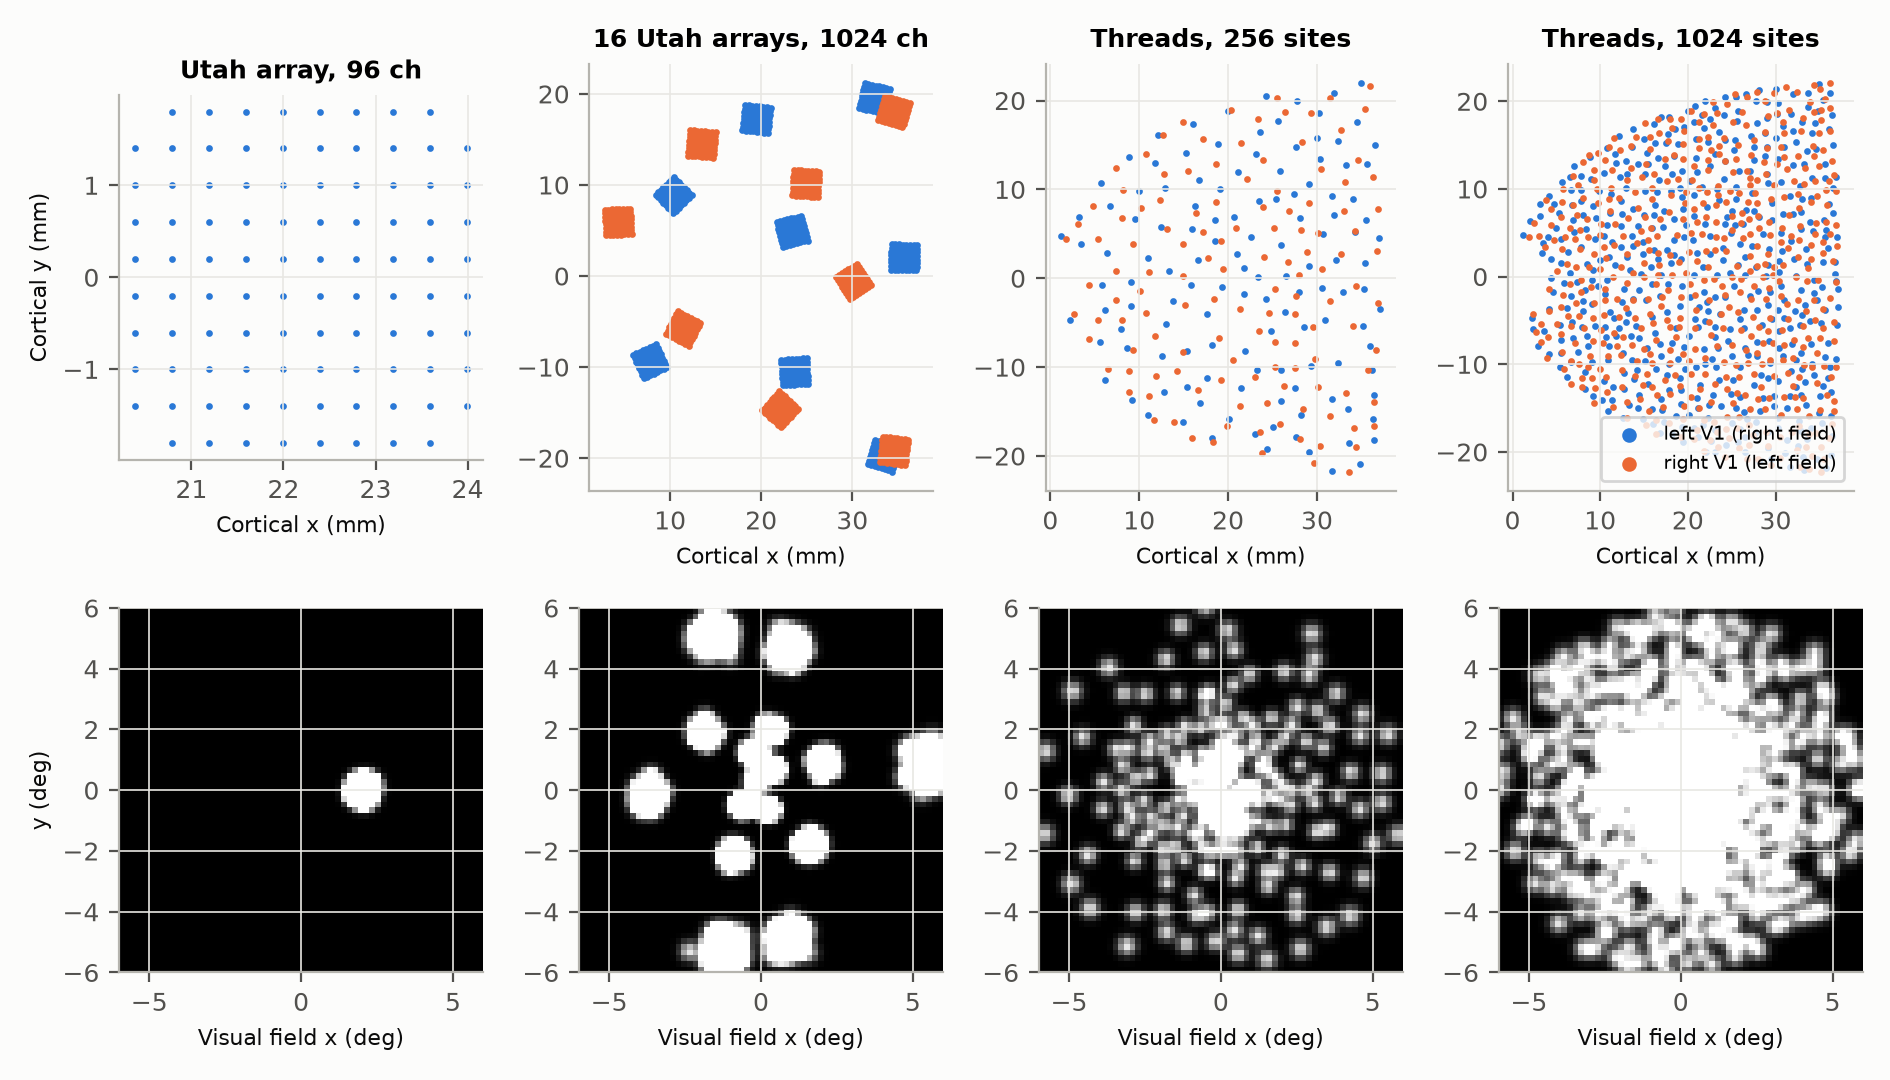
\includegraphics[width=0.85\textwidth]{fig_sim_layouts.png}
\caption{Electrode layouts on the flattened cortex (top row; blue = left V1, orange = right V1) and the percept of all electrodes at 80\,\textmu A for a held-out patient (bottom row).}
\label{fig:layouts}
\end{figure*}

\section{Stimulus encoders}\label{sec:enc}
Every encoder maps a $64{\times}64$ grayscale image spanning the $12^\circ$ field to amplitudes $a\in\mathbb R^N$. The amplitudes pass through a shared \textbf{safety layer} that clamps to $[0, I_{\max}{=}100\,\text{\textmu A}]$ (17\,nC/phase at 170\,\textmu s) and keeps at most $k{=}\lceil 0.25N\rceil$ active electrodes per frame. These stand in for charge-density and power/crosstalk budgets \citep{shannon1992model,cogan2008neural}.

\paragraph{Baselines.} All baselines sample a feature map bilinearly at each nominal phosphene centre. A sampled value $v_n\in[0,1]$ maps linearly from the electrode's (calibrated) threshold current to $I_{\max}$, and values $v_n\le0.1$ give zero current. The baselines are:
\begin{itemize}
\item \textbf{Intensity}: Gaussian-blurred image ($\sigma{=}1$\,px), in an \emph{uncalibrated} version (mean threshold, all electrodes assumed alive) and a \emph{calibrated} version;
\item \textbf{Edges}: Sobel magnitude;
\item \textbf{Salient edges}: Sobel magnitude weighted by spectral-residual saliency \citep{hou2007saliency}, a light-weight scene simplification \citep{han2021deep};
\item \textbf{Per-image optimisation}: for reference, amplitudes optimised separately for every image through the true patient simulator (100 Adam steps). This is non-causal and far too slow for real-time use.
\end{itemize}

\paragraph{Learned encoder.} The architecture has three stages:
\begin{enumerate}
\item A small U-Net (input image plus $x$, $y$ and eccentricity coordinate channels; resolutions 32 and 16; width 24) produces a stimulation map $s$ at half resolution.
\item The map is read out bilinearly at the nominal phosphene centres, $u_n=s(x_n,y_n)$.
\item The amplitude is $a_n=I_{\max}\,\mathrm{sigmoid}(g_n u_n+\beta_n)$.
\end{enumerate}
The network has \NumEncParams\ parameters for 1024 electrodes, because only the per-electrode gain and bias $(g_n,\beta_n)$ grow with $N$. The read-out uses only Gather operations, so the encoder exports to ONNX for in-browser and on-device inference.

\paragraph{Objective.} A decoder $D$ (a small CNN) reconstructs the image from the percept. With $\Phi=\mathcal S(\mathrm{Safety}(E(x));\text{patient})$:
\begin{multline}
\mathcal L = \|D(\Phi)-x\|^2 + \|\Phi-x\|^2 \\ + 0.5\,(1-\mathrm{SSIM}(\Phi,x)) + 0.05\,\overline{a/I_{\max}}.
\end{multline}
\begin{itemize}
\item The reconstruction term \citep{deruyter2022end} keeps the percept informative.
\item The percept terms keep it directly interpretable, since a person has no decoder.
\item The charge term discourages unnecessary stimulation.
\end{itemize}
We train with domain randomisation: the patient switches every 20 steps among 16 training patients that are disjoint from the test patients.

\paragraph{Patient adaptation.} After implantation, threshold mapping gives a calibrated forward model of that patient. We fine-tune a copy of the generic encoder for each patient, updating only the adapter $(g,\beta)$ (2$N$ parameters, decoder frozen). This uses 256 unlabeled images and 150 Adam steps. No labels or behavioural data are needed. We also compare against full fine-tuning with 16 to 1024 images.

\section{Experimental setup}
\begin{itemize}
\item \textbf{Data.} MNIST digits, EMNIST letters (26 classes; \citealp{cohen2017emnist}) and grayscale CIFAR-10 as a small natural-image proxy. Images are resized to $64{\times}64$ and fill the $12^\circ$ field.
\item \textbf{Training.} Encoders are trained on 20k training images for 1500 steps at batch size 32, with three seeds per dataset.
\item \textbf{Patients.} Evaluation uses five held-out patients (seeds 1000--1004) on the threads-1024 layout. Images are assigned to patients round-robin.
\item \textbf{Metrics.}
  \begin{itemize}
  \item SSIM \citep{wang2004image} and PSNR between percept and input.
  \item \emph{Low-pass SSIM}, computed after blurring both images with $\sigma{=}0.375^\circ$. Phosphene vision cannot carry detail finer than the phosphene spacing, and raw SSIM mostly scores dot texture.
  \item \emph{Recognition accuracy}: a fresh CNN is trained on each encoder's percepts of 6k training images (4 epochs) and tested on 2k test images. It stands in for a user who has learned that encoding \citep{rassia2018improvement}; the same CNN on the original images gives a ceiling.
  \item Stimulation cost: active electrodes per frame and summed charge per phase.
  \item Robustness: additional unannounced electrode failures (10/25/50\%), with no recalibration or retraining.
  \end{itemize}
\item \textbf{Compute.} Everything runs on a shared 8-core Intel CPU with 2 threads per process. A training run takes about \NumTrainMin\ minutes.
\end{itemize}
